\documentclass{article}
\usepackage{amsmath}
\usepackage{color,pxfonts,fix-cm}
\usepackage{latexsym}
\usepackage[mathletters]{ucs}
\DeclareUnicodeCharacter{46}{\textperiodcentered}
\DeclareUnicodeCharacter{305}{$\imath$}
\usepackage[T1]{fontenc}
\usepackage[utf8x]{inputenc}
\usepackage{pict2e}
\usepackage{wasysym}
\usepackage[english]{babel}
\usepackage{tikz}
\pagestyle{empty}
\usepackage[margin=0in,paperwidth=612pt,paperheight=792pt]{geometry}
\begin{document}
\definecolor{color_29791}{rgb}{0,0,0}
\begin{tikzpicture}[overlay]\path(0pt,0pt);\end{tikzpicture}
\begin{picture}(-5,0)(2.5,0)
\put(174.531,-166.608){\fontsize{17.2154}{1}\usefont{T1}{cmr}{m}{n}\selectfont\color{color_29791}Plan teamien to de la p r ob l em ´ atica}
\put(118.768,-238.408){\fontsize{14.3462}{1}\usefont{T1}{cmr}{b}{n}\selectfont\color{color_29791}Sistema gestor de solicitudes}
\put(118.768,-260.2289){\fontsize{9.9626}{1}\usefont{T1}{cmr}{m}{n}\selectfont\color{color_29791}En e l sistema que prop onemos u n usuario, seg ´ un su rol den tr o de la empresa, sea}
\put(118.768,-272.1839){\fontsize{9.9626}{1}\usefont{T1}{cmr}{m}{n}\selectfont\color{color_29791}capaz de generar solicitudes, a fin de p edir material, do cumen tos, man tenimien to}
\put(118.768,-284.1389){\fontsize{9.9626}{1}\usefont{T1}{cmr}{m}{n}\selectfont\color{color_29791}a m´ aquinas o to das aquellas transacc i o n e s que maneje el nego cio den tro de s ´ ı.}
\put(133.712,-296.0939){\fontsize{9.9626}{1}\usefont{T1}{cmr}{m}{n}\selectfont\color{color_29791}El sistema con tar´ a con roles esp ec ´ ıficos, con tar´ a tan to con un rol de admin-}
\put(118.768,-308.0499){\fontsize{9.9626}{1}\usefont{T1}{cmr}{m}{n}\selectfont\color{color_29791}istraci´ on que se encargar´ a de dar de alta a los n uev os usuarios, de actualizar}
\put(118.768,-320.0049){\fontsize{9.9626}{1}\usefont{T1}{cmr}{m}{n}\selectfont\color{color_29791}los cat´ alogos de op ciones de solicitud, y de v erificar los mo vimien tos den tro del}
\put(118.768,-331.9599){\fontsize{9.9626}{1}\usefont{T1}{cmr}{m}{n}\selectfont\color{color_29791}sistema. A su v ez, el sistema tend r´ a roles de empleado c omo sup ervisor, t ´ e cnico,}
\put(118.768,-343.9149){\fontsize{9.9626}{1}\usefont{T1}{cmr}{m}{n}\selectfont\color{color_29791}y empleado general.}
\put(133.712,-355.8698){\fontsize{9.9626}{1}\usefont{T1}{cmr}{m}{n}\selectfont\color{color_29791}Los empleados, sup ervisores y t ´ ecnicos con tar´ an con su propia vista, que les}
\put(118.768,-367.8248){\fontsize{9.9626}{1}\usefont{T1}{cmr}{m}{n}\selectfont\color{color_29791}dar´}
\put(134.3138,-387.1511){
\includegraphics[width=3.598491pt,height=3.838391pt]{latexImage_4914f52cf7a280ce3fc2532401a989af.png}}
\put(143.675,-387.7508){\fontsize{9.9626}{1}\usefont{T1}{cmr}{m}{n}\selectfont\color{color_29791}Los sup ervisores ser´ an capaces de acceder al registro de solicitudes hec has}
\put(143.675,-399.7058){\fontsize{9.9626}{1}\usefont{T1}{cmr}{m}{n}\selectfont\color{color_29791}en su departamen to/´ area y p o dr´ an aprobar o desaprobar las solicitudes}
\put(143.675,-411.6608){\fontsize{9.9626}{1}\usefont{T1}{cmr}{m}{n}\selectfont\color{color_29791}que}
\put(134.3138,-430.986){
\includegraphics[width=3.598491pt,height=3.838391pt]{latexImage_4914f52cf7a280ce3fc2532401a989af.png}}
\put(143.675,-431.5858){\fontsize{9.9626}{1}\usefont{T1}{cmr}{m}{n}\selectfont\color{color_29791}Los empleados de r ol “T ´ ecnico”, al acce d e r v er´ an los traba jos asignados}
\put(143.675,-443.5418){\fontsize{9.9626}{1}\usefont{T1}{cmr}{m}{n}\selectfont\color{color_29791}que el usuario com ´ un rep ort´ o con ob jeto de “Man tenimien t o” , y as ´ ı, ellos}
\put(143.675,-455.4968){\fontsize{9.9626}{1}\usefont{T1}{cmr}{m}{n}\selectfont\color{color_29791}p o d r´ an tomar resp onsabilidad de dic h as tareas in teractuando con esta}
\put(143.675,-467.4518){\fontsize{9.9626}{1}\usefont{T1}{cmr}{m}{n}\selectfont\color{color_29791}pan talla llev ando as ´ ı un registro de aquellos traba jos p endien tes o cerrados,}
\put(143.675,-479.4067){\fontsize{9.9626}{1}\usefont{T1}{cmr}{m}{n}\selectfont\color{color_29791}adem´}
\put(134.3138,-498.732){
\includegraphics[width=3.598491pt,height=3.838391pt]{latexImage_4914f52cf7a280ce3fc2532401a989af.png}}
\put(143.675,-499.3317){\fontsize{9.9626}{1}\usefont{T1}{cmr}{m}{n}\selectfont\color{color_29791}Los usuarios com unes p ueden solicitar div ersas cosas. Este formato, como}
\put(143.675,-511.2867){\fontsize{9.9626}{1}\usefont{T1}{cmr}{m}{n}\selectfont\color{color_29791}to dos, p o dr´ an encon trarlo en su “vista”.}
\put(133.712,-531.2127){\fontsize{9.9626}{1}\usefont{T1}{cmr}{m}{n}\selectfont\color{color_29791}Los empleados, en general, p o dr´ an acceder a su historial p ersonal de solici-}
\put(118.768,-543.1677){\fontsize{9.9626}{1}\usefont{T1}{cmr}{m}{n}\selectfont\color{color_29791}tudes generadas. Los sup ervisores p o dr´ an acceder al historial de solicitudes de}
\put(118.768,-555.1227){\fontsize{9.9626}{1}\usefont{T1}{cmr}{m}{n}\selectfont\color{color_29791}su ´ area.}
\put(133.712,-567.0777){\fontsize{9.9626}{1}\usefont{T1}{cmr}{m}{n}\selectfont\color{color_29791}Los t ´ ecnicos ser´ an capaces de acceder a las solicitudes en curso y p endien tes.}
\put(118.768,-579.0327){\fontsize{9.9626}{1}\usefont{T1}{cmr}{m}{n}\selectfont\color{color_29791}El t ´ ecnico, al tomar una solicitud, se compromete a darle resoluci´ on y no p o dr´ a}
\put(118.768,-590.9887){\fontsize{9.9626}{1}\usefont{T1}{cmr}{m}{n}\selectfont\color{color_29791}quedar como concluida hasta que el solicitan te aprueb e, den tro de su vista que}
\put(118.768,-602.9437){\fontsize{9.9626}{1}\usefont{T1}{cmr}{m}{n}\selectfont\color{color_29791}realmen te fue as ´ ı y puede con tin uar con sus actividades.}
\put(288.133,-692.6347){\fontsize{9.9626}{1}\usefont{T1}{cmr}{m}{n}\selectfont\color{color_29791}1}
\end{picture}
\newpage
\begin{tikzpicture}[overlay]\path(0pt,0pt);\end{tikzpicture}
\begin{picture}(-5,0)(2.5,0)
\put(118.768,-124.765){\fontsize{11.9552}{1}\usefont{T1}{cmr}{b}{n}\selectfont\color{color_29791}Captaci´ on de req uerimien tos}
\put(118.768,-143.154){\fontsize{9.9626}{1}\usefont{T1}{cmr}{m}{n}\selectfont\color{color_29791}El clien te solicitan te indica l os siguien tes pun tos como requisitos necesarios para}
\put(118.768,-155.109){\fontsize{9.9626}{1}\usefont{T1}{cmr}{m}{n}\selectfont\color{color_29791}el soft w are que a yudar´ a a su empresa:}
\put(130.945,-177.027){\fontsize{9.9626}{1}\usefont{T1}{cmr}{m}{n}\selectfont\color{color_29791}1. Quiere una vista de tip o administrad or con la que pueda dar de alta difer-}
\put(143.675,-188.982){\fontsize{9.9626}{1}\usefont{T1}{cmr}{m}{n}\selectfont\color{color_29791}en tes em p le ad os a tra v ´ es de una op ci´ on que se llame “Gesti´ on de usuarios”.}
\put(143.675,-200.937){\fontsize{9.9626}{1}\usefont{T1}{cmr}{m}{n}\selectfont\color{color_29791}T am bi ´ en deb e existir un historial donde pueda observ ar o consultar to das}
\put(143.675,-212.892){\fontsize{9.9626}{1}\usefont{T1}{cmr}{m}{n}\selectfont\color{color_29791}las solicitudes he c has p or to dos los empleados que han necesitado alg ´ un}
\put(143.675,-224.848){\fontsize{9.9626}{1}\usefont{T1}{cmr}{m}{n}\selectfont\color{color_29791}material. Aqu ´ ı mismo, tam b i ´ en quieren v er cuando se ha hec ho la solici-}
\put(143.675,-236.803){\fontsize{9.9626}{1}\usefont{T1}{cmr}{m}{n}\selectfont\color{color_29791}tud y que rol la ha hec ho. Cada solicitud deb e mostrar el estado en que}
\put(143.675,-248.7581){\fontsize{9.9626}{1}\usefont{T1}{cmr}{m}{n}\selectfont\color{color_29791}se encuen tra, si est´ a activ a, p endien te, rec hazada o aprobada.}
\put(130.945,-268.683){\fontsize{9.9626}{1}\usefont{T1}{cmr}{m}{n}\selectfont\color{color_29791}2. Una segunda vista p e r o que sea para los empleados donde ellos puedan}
\put(143.675,-280.638){\fontsize{9.9626}{1}\usefont{T1}{cmr}{m}{n}\selectfont\color{color_29791}llenar form u larios para realizar la solicitud de materiales. En los form u-}
\put(143.675,-292.594){\fontsize{9.9626}{1}\usefont{T1}{cmr}{m}{n}\selectfont\color{color_29791}larios deb en de mos tr ars e los datos de los empleados solicitan tes, datos}
\put(143.675,-304.549){\fontsize{9.9626}{1}\usefont{T1}{cmr}{m}{n}\selectfont\color{color_29791}como: nom bre, departamen to y rol. Las solicitudes se dividir´ an en 3 cat-}
\put(143.675,-316.504){\fontsize{9.9626}{1}\usefont{T1}{cmr}{m}{n}\selectfont\color{color_29791}egor ´ ıas: suministros, do cumen tos y man tenimien to. De igual manera, se}
\put(143.675,-328.459){\fontsize{9.9626}{1}\usefont{T1}{cmr}{m}{n}\selectfont\color{color_29791}mostrar´ a un historial para que los empleados puedan consul tar sus solici-}
\put(143.675,-340.414){\fontsize{9.9626}{1}\usefont{T1}{cmr}{m}{n}\selectfont\color{color_29791}tudes creadas y aclarar p osibles c on fusiones e inquietudes.}
\put(130.945,-360.34){\fontsize{9.9626}{1}\usefont{T1}{cmr}{m}{n}\selectfont\color{color_29791}3. Deb e hab er una tercera vista que sea para sup ervisores, aqu ´ ı los sup er-}
\put(143.675,-372.295){\fontsize{9.9626}{1}\usefont{T1}{cmr}{m}{n}\selectfont\color{color_29791}visores pueden v er un historial donde ellos recib en to das las solicitudes}
\put(143.675,-384.2499){\fontsize{9.9626}{1}\usefont{T1}{cmr}{m}{n}\selectfont\color{color_29791}elab oradas p or los empleados. Los sup ervisores se encargan de revisar}
\put(143.675,-396.2049){\fontsize{9.9626}{1}\usefont{T1}{cmr}{m}{n}\selectfont\color{color_29791}la informaci´ on de to das las solicitudes y ellos deciden qu ´ e solicitudes son}
\put(143.675,-408.1599){\fontsize{9.9626}{1}\usefont{T1}{cmr}{m}{n}\selectfont\color{color_29791}aprobadas y cu´ ales no. En caso d e requerirlo, los sup ervisores pueden}
\put(143.675,-420.1149){\fontsize{9.9626}{1}\usefont{T1}{cmr}{m}{n}\selectfont\color{color_29791}mo dificar solicitudes para su p osterior pro cesamien to. Cuando recib en}
\put(143.675,-432.0709){\fontsize{9.9626}{1}\usefont{T1}{cmr}{m}{n}\selectfont\color{color_29791}las solicitudes estas se encon trar´ an en estado p endien te y ellos pueden}
\put(143.675,-444.0259){\fontsize{9.9626}{1}\usefont{T1}{cmr}{m}{n}\selectfont\color{color_29791}cam biar su estado a rec hazada o ap robada.}
\put(130.945,-463.9509){\fontsize{9.9626}{1}\usefont{T1}{cmr}{m}{n}\selectfont\color{color_29791}4. Sistema de n otificaciones . Cada v ez que se le asigne una solicitud a un}
\put(143.675,-475.9059){\fontsize{9.9626}{1}\usefont{T1}{cmr}{m}{n}\selectfont\color{color_29791}empleado, y a se a t ´ ecnico o de man tenimien to, le ll e gar´ a una notifi c aci´ on}
\put(143.675,-487.8608){\fontsize{9.9626}{1}\usefont{T1}{cmr}{m}{n}\selectfont\color{color_29791}a su vista corresp ondien te.}
\put(288.133,-692.6348){\fontsize{9.9626}{1}\usefont{T1}{cmr}{m}{n}\selectfont\color{color_29791}2}
\end{picture}
\newpage
\begin{tikzpicture}[overlay]\path(0pt,0pt);\end{tikzpicture}
\begin{picture}(-5,0)(2.5,0)
\put(65.551,-582.093){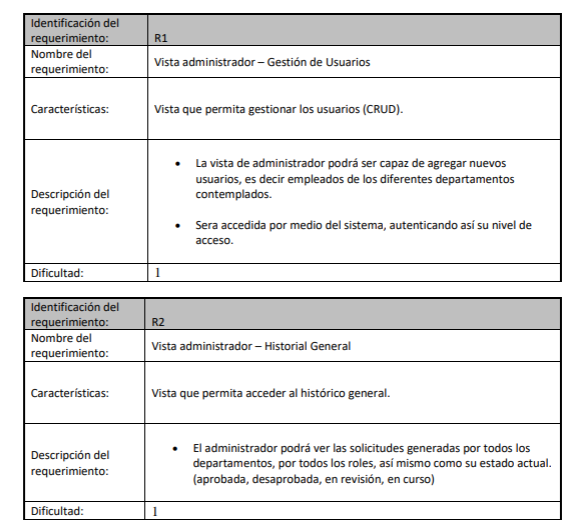
\includegraphics[width=446.8287pt,height=410.4949pt]{latexImage_b82d557265398c52c641ebc239515de5.png}}
\put(221.245,-604.011){\fontsize{9.9626}{1}\usefont{T1}{cmr}{m}{n}\selectfont\color{color_29791}Figure 1: Requerimien tos 1 y 2.}
\put(288.133,-692.635){\fontsize{9.9626}{1}\usefont{T1}{cmr}{m}{n}\selectfont\color{color_29791}3}
\end{picture}
\newpage
\begin{tikzpicture}[overlay]\path(0pt,0pt);\end{tikzpicture}
\begin{picture}(-5,0)(2.5,0)
\put(65.551,-601.854){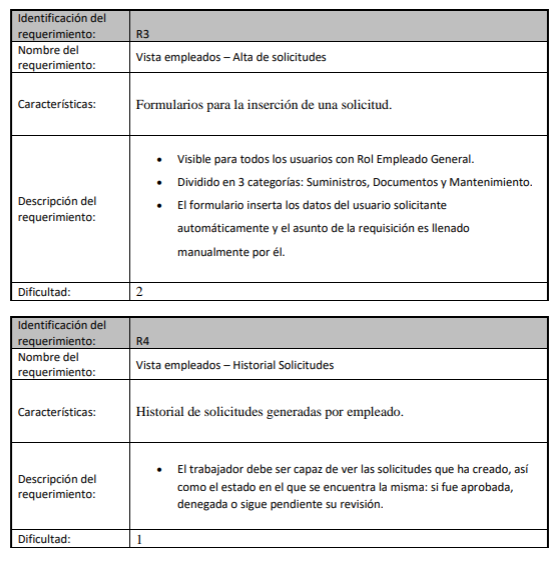
\includegraphics[width=446.824pt,height=450.0156pt]{latexImage_7ad2103c4684645d33079f183bef7275.png}}
\put(221.245,-623.771){\fontsize{9.9626}{1}\usefont{T1}{cmr}{m}{n}\selectfont\color{color_29791}Figure 2: Requerimien tos 3 y 4.}
\put(288.133,-692.635){\fontsize{9.9626}{1}\usefont{T1}{cmr}{m}{n}\selectfont\color{color_29791}4}
\end{picture}
\newpage
\begin{tikzpicture}[overlay]\path(0pt,0pt);\end{tikzpicture}
\begin{picture}(-5,0)(2.5,0)
\put(65.551,-606.968){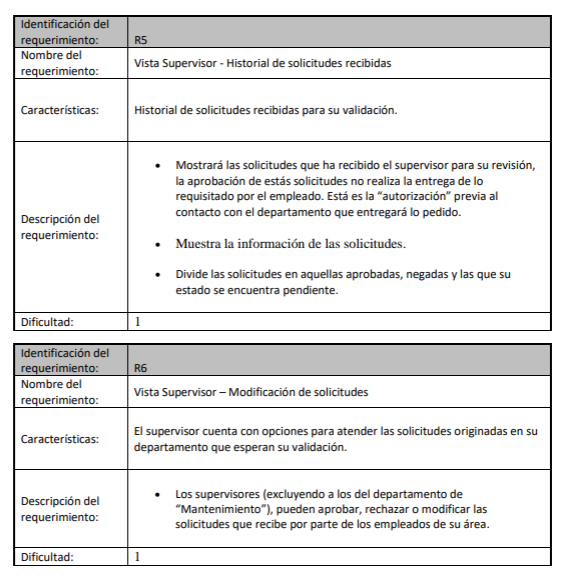
\includegraphics[width=446.847pt,height=460.2446pt]{latexImage_e973cf3a1511910abbe3939555bfcfdb.png}}
\put(221.245,-628.885){\fontsize{9.9626}{1}\usefont{T1}{cmr}{m}{n}\selectfont\color{color_29791}Figure 3: Requerimien tos 5 y 6.}
\put(288.133,-692.635){\fontsize{9.9626}{1}\usefont{T1}{cmr}{m}{n}\selectfont\color{color_29791}5}
\end{picture}
\newpage
\begin{tikzpicture}[overlay]\path(0pt,0pt);\end{tikzpicture}
\begin{picture}(-5,0)(2.5,0)
\put(65.551,-649.275){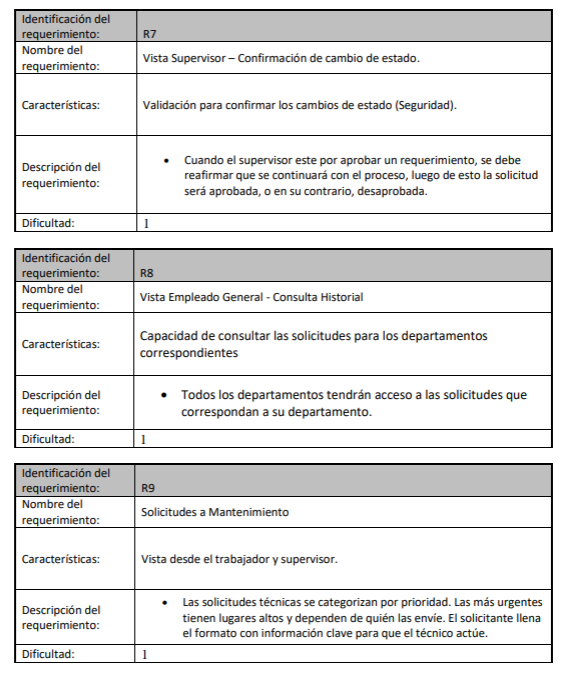
\includegraphics[width=446.84pt,height=534.4712pt]{latexImage_1d31847ef553f4cfb6b517b6b20d6348.png}}
\put(215.71,-671.193){\fontsize{9.9626}{1}\usefont{T1}{cmr}{m}{n}\selectfont\color{color_29791}Figure 4: Requerimien tos 7, 8 y 2.}
\put(288.133,-692.635){\fontsize{9.9626}{1}\usefont{T1}{cmr}{m}{n}\selectfont\color{color_29791}6}
\end{picture}
\newpage
\begin{tikzpicture}[overlay]\path(0pt,0pt);\end{tikzpicture}
\begin{picture}(-5,0)(2.5,0)
\put(65.551,-685.591){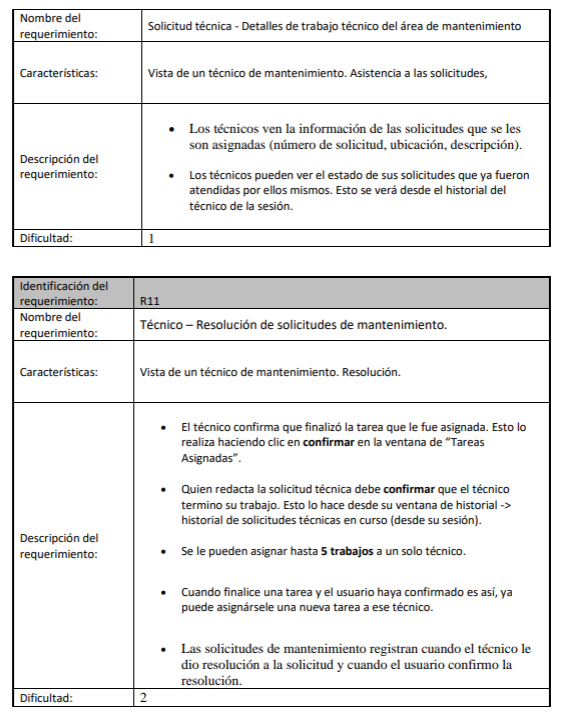
\includegraphics[width=446.84pt,height=570.7868pt]{latexImage_72a07b608896bb18c7decfd20592e3fd.png}}
\put(216.264,-707.508){\fontsize{9.9626}{1}\usefont{T1}{cmr}{m}{n}\selectfont\color{color_29791}Figure 5: Requerimien tos 10 y 11.}
\put(288.133,-692.635){\fontsize{9.9626}{1}\usefont{T1}{cmr}{m}{n}\selectfont\color{color_29791}7}
\end{picture}
\newpage
\begin{tikzpicture}[overlay]\path(0pt,0pt);\end{tikzpicture}
\begin{picture}(-5,0)(2.5,0)
\put(65.551,-609.406){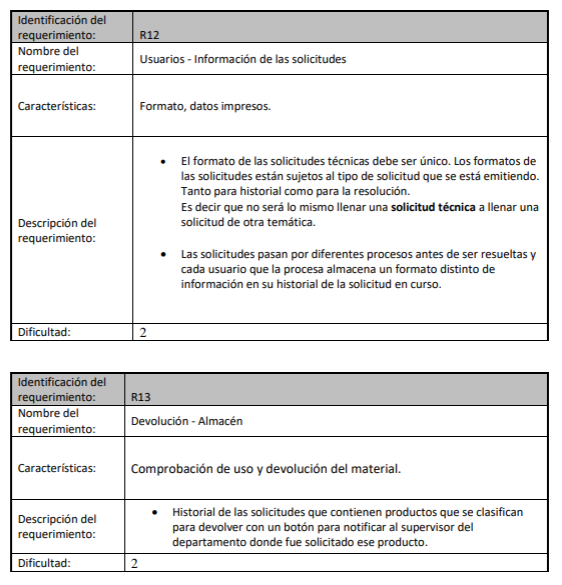
\includegraphics[width=446.8293pt,height=465.1159pt]{latexImage_27ead3e888a59e503511ba09428ac6dd.png}}
\put(216.264,-631.324){\fontsize{9.9626}{1}\usefont{T1}{cmr}{m}{n}\selectfont\color{color_29791}Figure 6: Requerimien tos 12 y 13.}
\put(288.133,-692.635){\fontsize{9.9626}{1}\usefont{T1}{cmr}{m}{n}\selectfont\color{color_29791}8}
\end{picture}
\newpage
\begin{tikzpicture}[overlay]\path(0pt,0pt);\end{tikzpicture}
\begin{picture}(-5,0)(2.5,0)
\put(65.551,-533.163){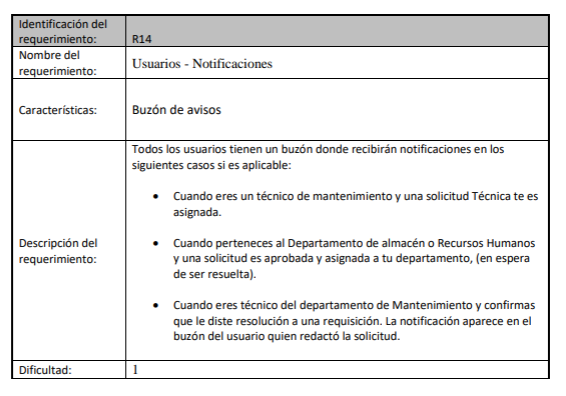
\includegraphics[width=446.84pt,height=312.6301pt]{latexImage_a81f1926e31b719e4cc2775db5fad9e5.png}}
\put(229.16,-555.08){\fontsize{9.9626}{1}\usefont{T1}{cmr}{m}{n}\selectfont\color{color_29791}Figure 7: Requerimien to 14.}
\put(288.133,-692.635){\fontsize{9.9626}{1}\usefont{T1}{cmr}{m}{n}\selectfont\color{color_29791}9}
\end{picture}
\newpage
\begin{tikzpicture}[overlay]\path(0pt,0pt);\end{tikzpicture}
\begin{picture}(-5,0)(2.5,0)
\put(65.551,-719.351){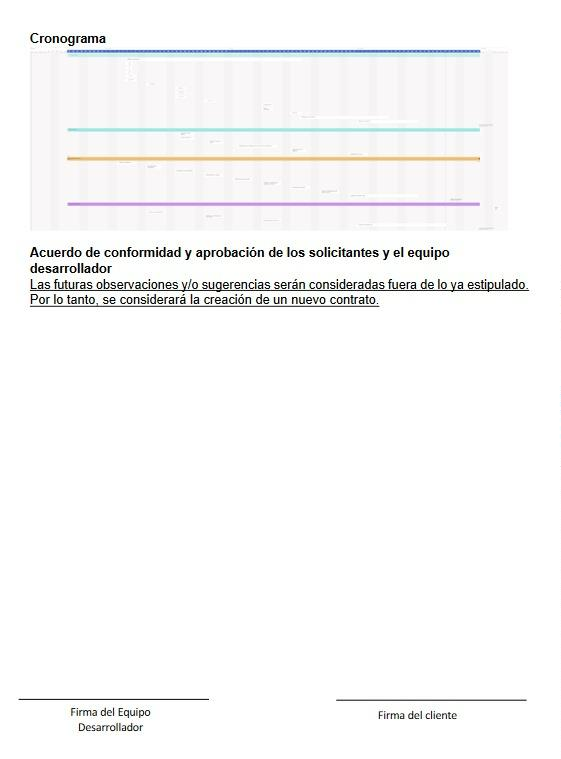
\includegraphics[width=446.8407pt,height=604.5492pt]{latexImage_e3c2f74adffecee60508e75784597752.png}}
\put(268.817,-741.268){\fontsize{9.9626}{1}\usefont{T1}{cmr}{m}{n}\selectfont\color{color_29791}Figure 8:}
\put(285.643,-692.635){\fontsize{9.9626}{1}\usefont{T1}{cmr}{m}{n}\selectfont\color{color_29791}10}
\end{picture}
\end{document}